\documentclass[a4paper]{article}

% Basic packages
\usepackage[fontset=fandol]{ctex}
\usepackage{amsmath, amssymb}
\usepackage{graphicx}
\usepackage[margin=2.5cm]{geometry}
\usepackage[most]{tcolorbox}
\usepackage{etoolbox}
\usepackage{listings}
\usepackage{hyperref}
\usepackage{booktabs}
\usepackage{subcaption}
\usepackage{float}
\usepackage{tikz}
\IfFileExists{pgfplots.sty}{
    \usepackage{pgfplots}
    \pgfplotsset{compat=1.18}
}{}

\newtcolorbox{knowledgebox}[1]{
    enhanced, colback=blue!5!white, colframe=blue!75!black, colbacktitle=blue!75!black,
    coltitle=white, fonttitle=\bfseries, title=#1, attach boxed title to top left={yshift=-2mm, xshift=2mm},
    boxrule=1pt, sharp corners
}

\newtcolorbox{importantbox}[1]{
    enhanced, colback=yellow!10!white, colframe=yellow!80!black, colbacktitle=yellow!80!black,
    coltitle=black, fonttitle=\bfseries, title=#1, sharp corners
}

\newtcolorbox{warningbox}[1]{
    enhanced, colback=red!5!white, colframe=red!75!black, colbacktitle=red!75!black,
    coltitle=white, fonttitle=\bfseries, title=#1, sharp corners
}

\lstset{
    language=Python,
    basicstyle=\ttfamily\small,
    keywordstyle=\color{blue},
    stringstyle=\color{red!60!black},
    commentstyle=\color{green!60!black},
    breaklines=true,
    frame=single,
    numbers=left,
    numberstyle=\tiny\color{gray},
    captionpos=b,
    extendedchars=false
}

\newcommand{\notetitle}{CME 295 第 6 讲：LLM Reasoning}
\newcommand{\noteauthors}{Codex 基于 Stanford CME 295 第 6 讲视频、字幕、讲稿与 slides 整理}
\newcommand{\notedate}{\today}
\newcommand{\videochannel}{Stanford CME 295}
\newcommand{\videopublishdate}{2025年11月7日课程录播}
\newcommand{\videoduration}{1:47:07}
\newcommand{\videourl}{https://www.youtube.com/watch?v=k5Fh-UgTuCo&list=PLoROMvodv4rOCXd21gf0CF4xr35yINeOy&index=6}
\newcommand{\videocoverpath}{cover.jpg}

\begin{document}

\begin{titlepage}
\centering
{\Large 课程笔记\par}
\vspace{1.2cm}
{\huge\bfseries \notetitle\par}
\vspace{0.8cm}
{\large \noteauthors\par}
\vspace{0.3cm}
{\large \notedate\par}
\vspace{1.2cm}

\ifdefempty{\videocoverpath}{
{\small 请在生成笔记时填入视频封面图的本地路径。\par}
}{
\includegraphics[width=0.82\textwidth,height=0.45\textheight,keepaspectratio]{\videocoverpath}\par
}

\vfill
\begin{tcolorbox}[width=0.9\textwidth, colback=black!2!white, colframe=black!60, sharp corners]
\textbf{视频作者/频道}：\videochannel\par
\textbf{发布日期}：\videopublishdate\par
\textbf{视频时长}：\videoduration\par
\textbf{视频链接}：
\href{\videourl}{\nolinkurl{\videourl}}
\end{tcolorbox}
\end{titlepage}

\tableofcontents
\newpage

\section{从 Vanilla LLM 到 Reasoning Model：问题到底变了什么}

\subsection{为什么课程先批判“普通 LLM”的边界}
Lecture 6 并不是一上来就讲 DeepSeek R1，而是先花不少时间说明 vanilla LLM 的强项和短板。课程承认，普通 LLM 已经非常擅长模仿、续写、生成代码和修 bug，也能在很多开放任务上给出看似不错的回答；但它们仍然存在几类明显问题：推理能力有限、知识静态、无法直接执行动作，而且自由文本输出很难评价。

老师这样铺垫的目的，是把“reasoning model”从营销标签还原成一个技术问题：如果普通 LLM 的训练目标主要是在已有分布上生成高似然文本，那么为什么它会天然擅长多步求解复杂问题？答案当然是不会。因此 reasoning model 不是普通助手的简单加强版，而是围绕“多步求解”重新组织训练与评测目标的产物。

\subsection{课程对 reasoning 的工作定义}
Slides 明确说，并没有一个全行业统一认可的 reasoning 定义。课程给出的工作定义是：\textbf{reasoning 是解决问题的能力，尤其是需要多步中间过程的问题。} 这里典型例子是数学题、代码题、逻辑题，而不是直接从记忆里取出一个事实。

老师还给出了一组对照：像“Stanford 这门课的课程代码是什么”更像是检索式问题，而“这只熊 2020 年出生，现在 2025 年，几岁了”则需要显式中间步骤。这个区分非常关键，因为它说明 reasoning 并不等同于“回答正确”，而是和问题是否需要分解、推演、验证直接相关。

\subsection{新范式：输出不再只有答案，还包含推理链}
课程把 reasoning model 的核心转向画得很直白：过去是 \texttt{Question -> LLM -> Answer}，现在变成 \texttt{Question -> LLM -> Reasoning chain + Answer}。也就是说，模型被鼓励先产生中间推理，再给最终答案。

\begin{figure}[H]
\centering

\includegraphics[width=0.9\textwidth]{pdf_pages/page-24.png}
\caption{Reasoning model 的新范式：输出不仅包含最终答案，还显式包含中间 reasoning chain。}
\end{figure}

这一变化的技术意义非常大。它把原本隐含在模型内部的“求解过程”变成显式可训练、可奖励、可控制的对象。后面所有 test-time scaling、verifiable reward、GRPO 和 R1 训练 recipe，都是在围绕这条“让推理链可优化”展开。

\subsection{本章小结}
Lecture 6 的第一步是澄清问题：reasoning model 不是“更强聊天机器人”这么简单，而是把多步求解过程显式化的模型。只有先承认 vanilla LLM 的能力边界，后面关于 reasoning training 的设计才有意义。

\section{评测与表征：怎样判断模型真的更会推理了}

\subsection{Reasoning 任务最常见的两大载体：代码和数学}
Slides 给出的 benchmark 景观非常典型。代码方向上，课程提到 HumanEval、CodeForces、SWE-bench；数学方向上则提到 AIME、GSM8K 等。这些任务共同特点是：它们都要求模型不是简单“说得像”，而是要真的给出可检查的结果，比如通过测试用例、得到正确数值答案、或完成逻辑推导。

从教学角度看，课程想让学生注意的是：reasoning benchmark 往往有某种\textbf{可验证性}。这和开放式聊天质量不同，因为系统可以较客观地判断答案是否正确，也因此更适合作为 RL 奖励的来源。

\subsection{Pass@k 与 Cons@k：为什么 reasoning 评测经常不是单次命中率}
Lecture 6 特别回顾了 code benchmark 里常见的 Pass@k。其含义是：如果允许模型尝试 $k$ 次，至少有一次成功的概率是多少。对于能自动验证的任务，这个指标非常合理，因为真实系统可以多采样、跑测试、再选最好结果。

Slides 还提到 Pass@1 与 Cons@k。Pass@1 对应“只生成一次就要尽量答对”的场景；Cons@k 则强调多次采样后的一致性或共识。这些指标共同说明，reasoning model 的评测和普通聊天模型不同，它不一定只关心单次输出，而经常关心“多次尝试 + 可验证选择”这一整套流程。

\begin{knowledgebox}{Lecture 6 的评测观}
如果一个任务的验证器足够可靠，那么系统不必把全部赌注押在一次采样上。Pass@k 之类指标正是把“可多次尝试、可自动检查”的现实工作流编码进评测方式里。
\end{knowledgebox}

\subsection{课程为什么强调 reasoning model 是近一年才爆发的主题}
字幕里老师反复提到，这一讲的大部分材料都来自 2024 或 2025 年，非常新。这一提醒有两层含义：第一，很多方法仍在快速演化，没有最终定论；第二，现在回头看已经能分辨哪些东西只是热闹，哪些东西真的构成了 reasoning training 的稳定骨架。Lecture 6 选择聚焦的，就是后者。

\subsection{本章小结}
Reasoning model 的评测通常依赖代码、数学这类可验证任务，指标也往往从单次准确率扩展到 Pass@k、Cons@k 等多采样视角。这为后续引入“可验证奖励”提供了非常自然的桥梁。

\section{可验证奖励与 Test-Time Scaling：让模型愿意多想、还能被检查}

\subsection{为什么 reasoning chain 不能完全依赖人工写 SFT 数据}
进入训练方法后，课程首先指出一个现实问题：高质量 reasoning chain 很难大规模人工撰写。如果完全依赖人工构造长链式推理数据，不仅昂贵，还可能把模型限制在人类现有的写法里，抑制模型探索更高效或更奇特的推理路径。这就是为什么 reasoning 训练很快转向 RL。

\subsection{可验证奖励的核心：格式 + 正确性}
Lecture 6 引入了 \textbf{verifiable rewards} 的概念。Slides 先给出一个极简模板：模型需要按照某种带有 \texttt{<think>} 分隔符的格式输出推理，再给出最终答案。于是奖励可以拆成两部分：
\[
r = r_{\mathrm{format}} + r_{\mathrm{acc}}.
\]

符号说明如下：
\begin{itemize}
\item $r$：总奖励；
\item $r_{\mathrm{format}}$：格式奖励，检查是否按约定输出推理链或分隔符；
\item $r_{\mathrm{acc}}$：正确性奖励，检查最终答案是否通过测试或数值校验。
\end{itemize}

\begin{figure}[H]
\centering

\includegraphics[width=0.84\textwidth]{pdf_pages/page-61.png}
\caption{课程把 reasoning RL 的奖励拆成两部分：格式是否符合约定，以及答案是否可验证地正确。}
\end{figure}

这套设计非常漂亮，因为它不依赖人工逐句评价 reasoning chain，而是利用程序化验证器去判断“有没有推理结构”和“结果对不对”。对于代码题，这个验证器可以是测试用例；对于数学题，可以是自动判题器或规则校验器。

\subsection{Test-time scaling 的真正含义}
课程把“test-time scaling”解释成：在推理阶段显式给模型更多思考空间，鼓励它通过更长的 reasoning chain 去提升最终正确率。这里的关键不是简单多生成 token，而是让额外 token 尽可能服务于求解过程。

Slides 随后讨论了几种控制思考预算的方式：dynamic budget、context awareness、budget forcing，以及更一般的“连续思考”思路。老师想表达的是，不同问题并不需要同样长的推理链；reasoning model 的一个高级能力，就是知道什么时候该多想，什么时候该尽快作答。

\begin{importantbox}{多想不等于乱想}
Test-time scaling 的目标不是无条件拉长输出，而是让模型把额外计算预算用于有价值的中间推理。否则，长输出只会增加成本和噪声，而不提高正确率。
\end{importantbox}

\subsection{本章小结}
Reasoning 训练之所以适合 RL，很大程度上是因为存在可验证奖励。只要能够自动检查格式和正确性，模型就可以在较少人工监督下不断试错，并把“多想一点”变成可学习的行为。

\section{GRPO 与长度偏置：Reasoning RL 为什么和 PPO 不一样}

\subsection{GRPO 的核心改动：用组内平均回报做基线}
Lecture 6 选择 GRPO 作为 reasoning 训练中的代表算法。它与 PPO 的相似点在于，仍然保留 ratio、clipping 和对参考策略的约束；但最大的差异是 advantage 的估计方式不同。GRPO 不再依赖单独的 value model，而是使用同一组候选回答的平均奖励作为基线：
\[
A_i = r_i - \frac{1}{G}\sum_{j=1}^{G} r_j.
\]

符号说明如下：
\begin{itemize}
\item $A_i$：第 $i$ 个候选回答的 group-relative advantage；
\item $r_i$：第 $i$ 个候选回答的奖励；
\item $G$：同一 prompt 下采样得到的候选数量；
\item $\frac{1}{G}\sum_{j=1}^{G} r_j$：该组候选回答的平均奖励。
\end{itemize}

这个设计的直觉很自然：对于同一问题，哪个回答比同组其他回答更好，就鼓励哪个；不需要额外训练一个 value function 去预测 baseline。

\begin{figure}[H]
\centering

\includegraphics[width=0.9\textwidth]{pdf_pages/page-94.png}
\caption{Slides 直接对比 GRPO 与 PPO，强调两者的差异主要集中在 advantage estimation 和 KL 处理方式。}
\end{figure}

\subsection{为什么 GRPO 很适合 reasoning 场景}
对于 reasoning 任务，同一个 prompt 下往往可以采样出多条不同推理链，而且这些链的好坏能通过自动验证器判断。于是“组内相对比较”就非常自然：不必估计绝对价值，只需判断在这一组候选里谁表现更好。课程借此说明，GRPO 的成功并不是偶然，而是与 reasoning 任务的候选生成和可验证评测天然契合。

\subsection{输出长度为什么会越训越长}
课程随后指出一个非常关键的副作用：\textbf{increasing output length phenomenon}。随着 RL 训练推进，模型可能越来越倾向于输出更长的 reasoning chain。原因不是它一定学会了更深的推理，而是目标函数和 token 级归一化可能诱导了“多写一点也许更有利”的坏激励。

Slides 用公式页强调了长度相关项的影响。直观上，如果长输出里的每个 token 贡献被平均稀释，那么在某些情形下，模型可能通过延长输出把负面 token 的惩罚摊薄，形成错误激励。这不是 reasoning 提升，而是目标设计漏洞。

\begin{figure}[H]
\centering

\includegraphics[width=0.9\textwidth]{pdf_pages/page-105.png}
\caption{课程把长度偏置直观化：不恰当的 token 级归一化可能让“更长输出”获得不合理优势。}
\end{figure}

\subsection{DAPO、Dr. GRPO 与其他修正}
为了缓解长度膨胀问题，Lecture 6 列出了 DAPO、Dr. GRPO 等改进方向。它们大体思路都是重写 token 贡献方式，使长输出和短输出的奖励分配更公平，减少“单纯拉长文本”带来的虚假收益。课程还提到其他调整，例如降低难度偏置、鼓励多样性等，说明 reasoning RL 仍然在快速迭代，许多训练细节尚未完全定型。

\begin{warningbox}{为什么这一节很重要}
如果只看 headline，很容易以为 reasoning RL 的秘诀就是“上 GRPO”。但课程真正想强调的是：奖励设计、归一化方式和长度激励同样关键。算法名字只是骨架，训练细节决定行为。
\end{warningbox}

\subsection{本章小结}
GRPO 通过组内平均奖励构造 advantage，省掉了 value model，也更贴合 reasoning 的多候选可验证场景。但一旦目标函数设计不慎，就会出现输出长度失控等副作用，因此 reasoning RL 的难点仍然在奖励与归一化细节上。

\section{DeepSeek R1 系列与 Distillation：把推理能力真正做成一条训练流水线}

\subsection{R1-Zero：只靠 RL 就能逼出推理行为，但还不够产品化}
课程先讲 DeepSeek R1-Zero。其基本 recipe 是：先有一个强大的基础模型 V3-Base，再直接在 reasoning 数据上用 GRPO 做强化学习，从而诱导模型学会生成推理链。Slides 给出的好处包括：不依赖人工 SFT reasoning data，也能浮现出明显推理能力；但缺点同样突出，例如推理链格式混乱、语言不稳定、可读性和可控性不足。

这一步的教学意义在于说明：\textbf{reasoning 行为确实可以通过 RL 从可验证奖励中直接长出来。} 但如果想把它做成稳定、可部署、兼顾通用交互质量的系统，仅靠一轮 RL 还不够。

\subsection{R1：把 SFT 与 RL 重新交错起来}
接下来课程给出 DeepSeek R1 的完整 recipe。它不是简单“多跑一点 RL”，而是把预训练、小规模 reasoning SFT、GRPO、大规模混合 SFT 和最终 GRPO 再次串起来，形成多阶段流水线。课程强调，这条流水线既保留了 RL 对 reasoning 行为的塑造能力，也重新引入了 SFT 对语言质量和可控性的整形作用。

\begin{figure}[H]
\centering
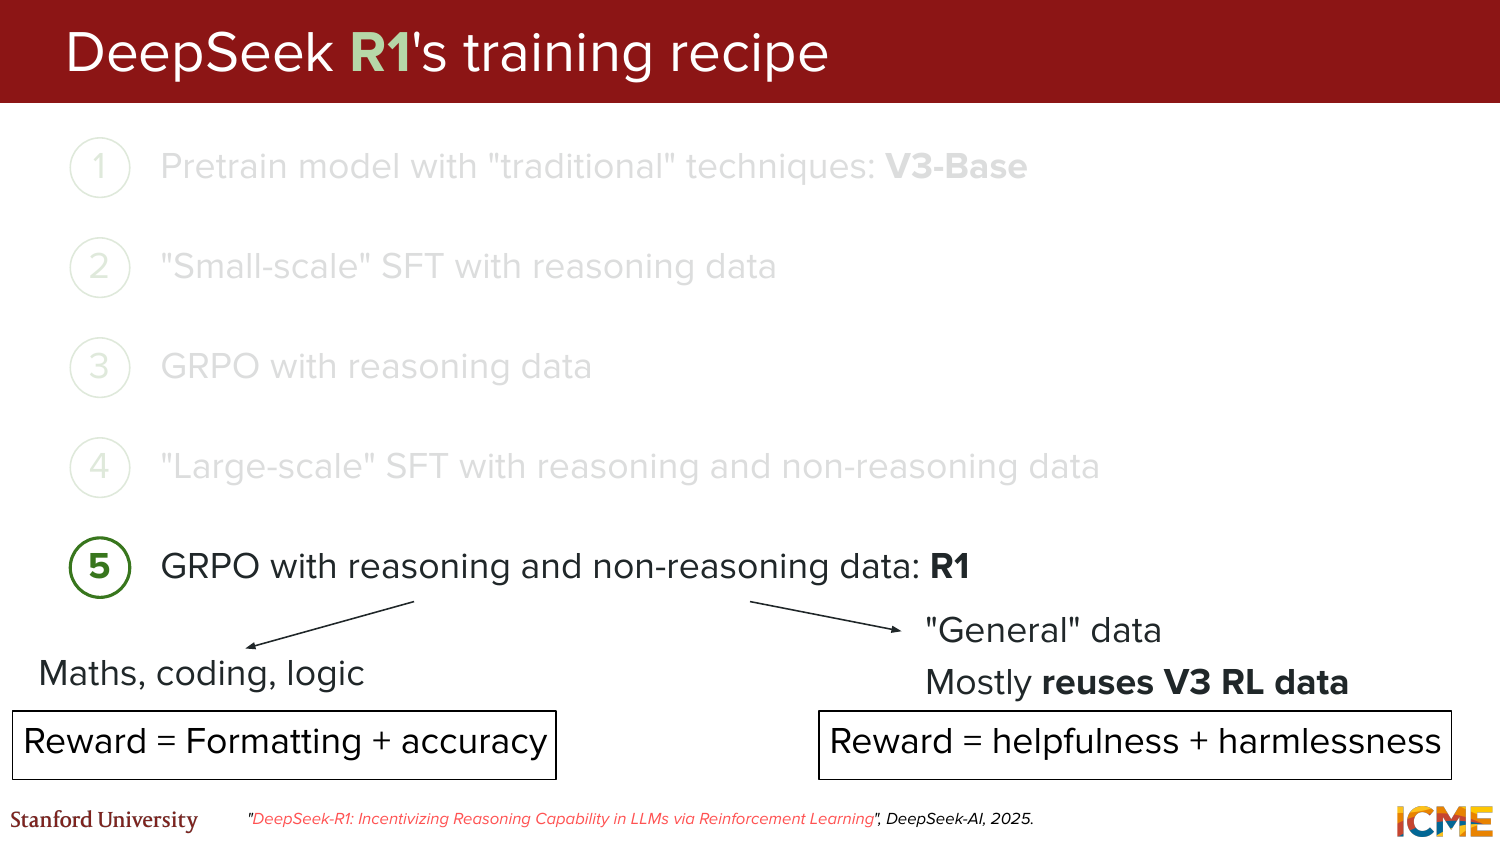
\includegraphics[width=0.9\textwidth]{pdf_pages/page-138.png}
\caption{DeepSeek R1 的后段 recipe 强调：在 reasoning 与 non-reasoning 数据上继续做 GRPO，使模型兼顾推理、帮助性与安全性。}
\end{figure}

尤其值得注意的是，Slides 在第 5 步把数据分成两类：数学、代码、逻辑这类 reasoning-heavy 数据，以及更通用的“general”数据。前者主要奖励格式和正确性，后者则奖励 helpfulness 与 harmlessness。这说明产品级 reasoning model 并不是只会做题，而是要把“会想”与“会交流”重新兼容起来。

\subsection{Distillation：把 reasoning traces 蒸馏给更小模型}
Lecture 6 的最后一个重点是 distillation。课程刻意对比了 lecture 2 里传统 distillation 和这里的新用法。传统蒸馏的目标是让学生模型去匹配教师模型的 next-token 分布；而在 reasoning 语境里，蒸馏更像是让学生模型直接学习教师生成的完整 reasoning traces。

\begin{figure}[H]
\centering
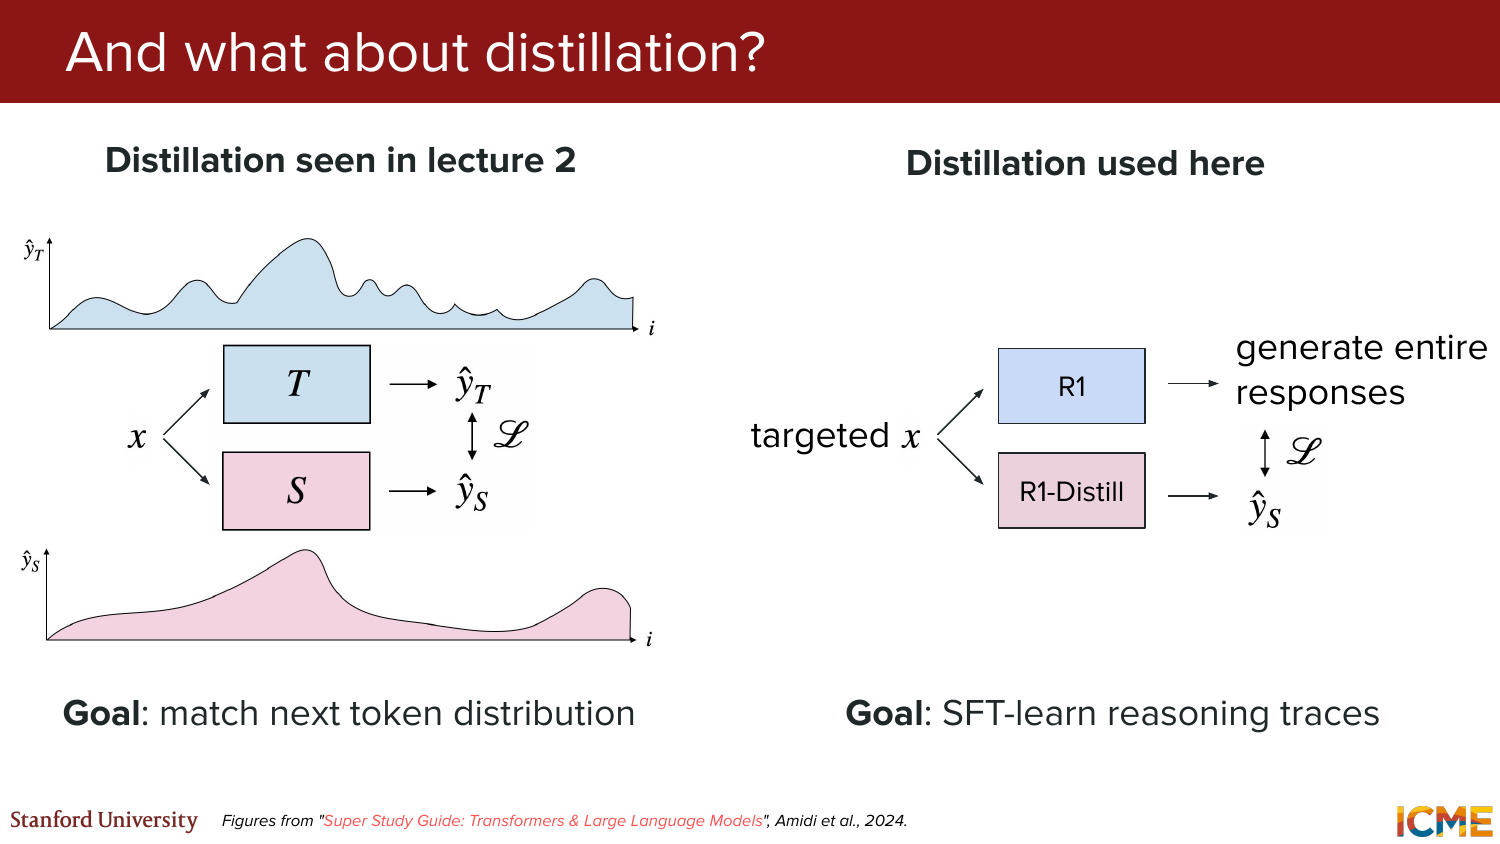
\includegraphics[width=0.9\textwidth]{pdf_pages/page-144.png}
\caption{课程对比了传统 distillation 与 reasoning distillation：后者不只是匹配分布，而是让学生模型学习完整推理轨迹。}
\end{figure}

这一步的意义非常现实。前沿 reasoning model 往往训练代价极高、推理成本也高，如果能够把其推理轨迹蒸馏给更小模型，就可能在成本和效果之间取得更好的工程折中。Slides 也给出结论：这种做法常常能得到相当有竞争力的结果，而且是一种“更划算地使用算力”的方式。

\subsection{本章小结}
DeepSeek R1 系列说明，reasoning model 不是一招鲜，而是一条组合式流水线：预训练提供基座，RL 逼出 reasoning 行为，SFT 修语言和格式，再用混合奖励把 reasoning 与通用助手能力重新整合。Distillation 则把这套能力继续压缩到更便宜的模型上，形成产业上可复制的路径。

\section{总结与延伸}
Lecture 6 把 reasoning model 这件事拆解得非常清楚。首先，课程从 vanilla LLM 的能力边界出发，重新定义 reasoning 是多步求解问题的能力，而不是简单事实回忆。接着，课程说明 reasoning 任务之所以适合 RL，是因为代码和数学场景通常拥有可验证奖励，从而可以把“格式是否正确”“答案是否正确”写成自动化评分信号。随后，GRPO 作为 reasoning RL 的代表方法登场，用组内平均奖励替代 value model；而长度膨胀问题又提醒我们，真正困难的不只是选算法，还包括奖励设计和归一化细节。最后，DeepSeek R1-Zero、R1 与 distillation 展示了一条更完整的工程路线：RL 让推理能力浮现，SFT 让交互更可控，混合数据和混合奖励让模型既会推理又能当通用助手，而蒸馏则把这套能力下放到成本更低的模型。

如果把 Lecture 5 和 Lecture 6 连起来看，一个很清楚的趋势会浮现出来：偏好学习和 RL 不再只是用来让模型“更礼貌、更安全”，而是被进一步用来塑造更强的推理过程。换句话说，reasoning model 并不是凭空冒出来的新物种，而是建立在 SFT、RLHF、DPO、可验证奖励和 test-time scaling 这一整串方法之上的下一阶段产物。

\end{document}
